\documentclass[a4paper, 10pt, conference]{ieeeconf}

\IEEEoverridecommandlockouts
\overrideIEEEmargins

\usepackage{graphics} % for pdf, bitmapped graphics files
\usepackage{epsfig} % for postscript graphics files
\usepackage{mathptmx} % assumes new font selection scheme installed
\usepackage{times} % assumes new font selection scheme installed
\usepackage{amsmath} % assumes amsmath package installed
\usepackage{amssymb}  % assumes amsmath package installed
\usepackage{hyperref}
\usepackage{listings}
\usepackage{subfigure}

\usepackage[T1]{fontenc}
\usepackage[utf8]{inputenc}
\usepackage[brazil]{babel}
\usepackage{etoolbox}
\patchcmd{\abstract}{Abstract}{Resumo}{}{}
\patchcmd{\thebibliography}{References}{Referências}{}{}

\title{\LARGE \bf Otimizando o tempo de execução no processamento de imagens}

\author{Henrique Miyamoto e Thiago Benites \thanks{* Os arquivos do projeto estão disponíveis em \url{https://github.com/miyamotohk/linguagem-processamento-imagem}.}}

\begin{document}
\maketitle
\thispagestyle{empty}
\pagestyle{empty}

%\begin{abstract}

%Escreva aqui o resumo (abstract).

%\end{abstract}

\section{Contextualização}

%Um breve texto introdutório explicando do que se trata o documento, em uma linguagem que poderia ser entendida por qualquer pessoa que entenda programação (ou seja: referências diretas à disciplina não são desejáveis).

\textit{Threads}, assim como processos, são mecanismos que permitem que um programa execute ações de forma aparentemente simultânea. A diferença é que \textit{threads} possuem área de memória compartilhada, o que não ocorre com processos \cite{alp}. Apresentamos uma comparação de desempenho entre diferentes métodos para aplicação de brilho em uma imagem: usando múltiplas \textit{threadas}, usando multiprocessos, em uma única linha de execução, varrendo a matriz por linhas e por colunas. O objetivo é comparar e discutir os desempenhos de cada implementação a partir do tempo de execução real e de usuário de cada uma delas.

%A tabela \ref{tabela1} apresenta as sintaxes para os diferentes métodos de aplicação de brilho usados em nosso programa.

%\begin{table}[h]
%	\centering
%	\caption{Sintaxe para diferentes métodos de aplicação de brilho}
%	\label{tabela1}
%	\begin{tabular}{|c|c|}
%		\hline \textbf{Método de implementação} & \textbf{Sintaxe}\\
%		\hline \textit{Multithreadas} & \begin{tabular}[c]{@{}c@{}}{destino.jpg = origem.jpg *float THR int}\end{tabular} \\
%		\hline Multiprocessos & \begin{tabular}[c]{@{}c@{}}{destino.jpg = origem.jpg *float PRC int}\end{tabular} \\ 
%		\hline Varredura por linhas & \begin{tabular}[c]{@{}c@{}}{destino.jpg = origem.jpg *float LIN}\end{tabular} \\ 
%		\hline Varredura por colunas & \begin{tabular}[c]{@{}c@{}}{destino.jpg = origem.jpg *float COL}\end{tabular} \\ 
%		\hline
%	\end{tabular}
%\end{table}

\section{Demonstração}

%Entradas e saídas que demonstram as funcionalidades implementadas.

Na comparação de desempenho, foram usadas imagens pequena (32x32 pixels), média (720x460) e grande (2592x1944) e foram medidos os tempos reais (tempo de relógio) e de usuário (tempo que a CPU gasta dentro dos processos). O processador usado para os testes tinha as seguintes especificações: \textit{Intel(R) Core(TM) i5-7200U CPU @ 2.50GHz}.

Inicialmente, variou-se a quantidade de \textit{threads} e processos em cada execução para otimizar esse número. Nesse procedimento, a imagem média foi usada como referência. A otimização do tempo de execução se dá para aproximadamente 800 \textit{threads} e 1 processo, dentre os resultados avaliados.

\begin{figure}[h]
	\centering
	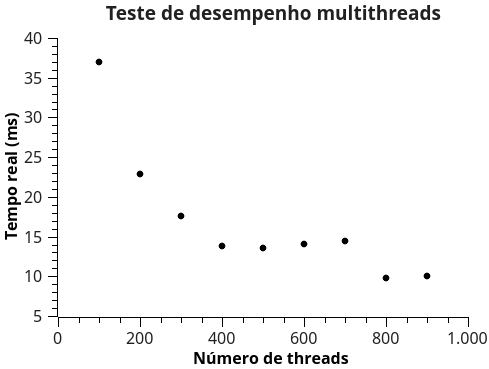
\includegraphics[width=3.65cm]{Figuras/multithreads}
	\caption{Tempo real (ms) em função do número de \textit{threads}.}
\end{figure}

\begin{figure}[h]
	\centering
	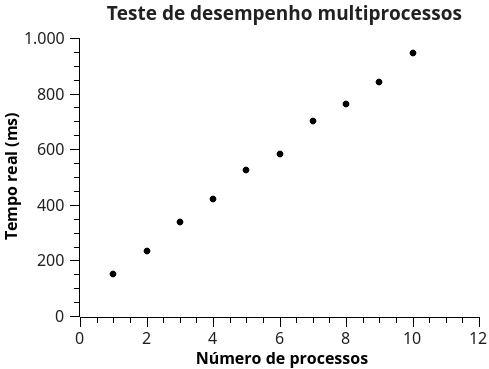
\includegraphics[width=3.65cm]{Figuras/multiprocessos}
	\caption{Tempo real (ms) em função do número de multiprocessos.}
\end{figure}

A seguir, foram comparados os diferentes métodos de aplicação de brilho para cada imagem. Nesse teste, o número de \textit{threads} e processos usados foi o número ótimo encontrado anteriormente.

\begin{table}[h]
	\centering
	\caption{Testes de desempenho para imagens pequena, média e grande}
	\label{my-label}
	\begin{tabular}{|c|c|c|c|}
		\hline
		\textbf{Método}       & \textbf{Tamanho} & \textbf{Tempo real} & \textbf{Tempo de usuário} \\ \hline
		\textit{Multithreads}          & 32x32            & 0,6650 ms           & 0,3650 ms                 \\
		Multiprocessos        & 32x32            & 5,8270 ms           & 5,8280 ms                 \\
		Varredura por colunas & 32x32            & 0,0310 ms           & 0,0300 ms                 \\
		Varredura por linhas  & 32x32            & 0,0210 ms           & 0,0200 ms                 \\ \hline
		\textit{Multithreads}          & 720x460          & 9,4800 ms           & 2,5760 ms                 \\
		Multiprocessos        & 720x460          & 147,2950 ms         & 65,1070 ms                \\
		Varredura por colunas & 720x460          & 9,2150 ms           & 9,2150 ms                 \\
		Varredura por linhas  & 720x460          & 6,8940 ms           & 6,8930 ms                 \\ \hline
		\textit{Multithreads}          & 2592x1944          & 135,3250 ms         & 39,6660 ms                \\
		Multiprocessos        & 2592x1944          & 3819,1140 ms        & 637,9850 ms               \\
		Varredura por colunas & 2592x1944          & 149,0920 ms         & 149,0950 ms               \\
		Varredura por linhas  & 2592x1944          & 142,3600 ms         & 142,3610 ms               \\ \hline
		
	\end{tabular}
\end{table}


\section{Análise}

%Aqui deve-se comparar a qualidade, em questão de tempo, de cada implementação. Ademais, analisar-se-ão quais métodos são vantajosos de acordo com diferentes tamanhos de imagens e de pixels fixados para análise por função.

Observa-se que o método com menor tempo real de execução depende do tamanho da imagem utilizada. Para as imagens pequena e média, a varredura em uma única linha de execução por linhas apresenta melhor desempenho. Já para a imagem grande, este é alcançado pelo método \textit{multithreads}. Uma explicação para essa diferença é a solução de compromisso inerente ao procedimento \textit{multithreads}: existe um gasto computacional para a criação das threads, que só é compensado para imagens muito grandes, para as quais a execução paralela é vantajosa.

A implementação com múltiplos processos mostrou desempenho inferior às demais implementações. É possível que esse fato esteja relacionado ao gasto computacional necessário para criação da área de memória compartilhada e criação individual de cada processo. Em todos os casos, a varredura por linha apresentou tempo menor que por colunas, fato derivado de como a matriz foi definida. As linhas são posicionadas em sequência, logo, a análise se dá consecutivamente, pixel a pixel, enquanto que em colunas, não há essa sequência na posição de cada pixel.

Nos casos em que o tempo real é menor que o tempo de usuário, a aplicação do brilho é \textit{CPU bounded} (i.e., o maior gargalo de execução está no processador). Por outro lado, no caso contrário, é \textit{I/O bounded} (i.e., o gargalo está na entrada/saída de dados), pois o programa passa tempo esperando os dados.

\begin{thebibliography}{99}

\bibitem{alp} MITCHELL, Mark; OLDHAM, Jeffrey e SAMUEL, Alex. \textit{Advanced Linux Programming}. Indianopolis: New Riders, 2001.

\end{thebibliography}

\end{document}